\section{Work Breakdown and Schedule}
A work breakdown structure (WBS) is important to understand the complexity of the project and how components are structured. This information is particularly useful for agile development, so that releases can be scheduled based on a selection of the WBS,
 such that each component requires roughly the amount of time available in one development cycle.

\begin{figure*}[h!]
	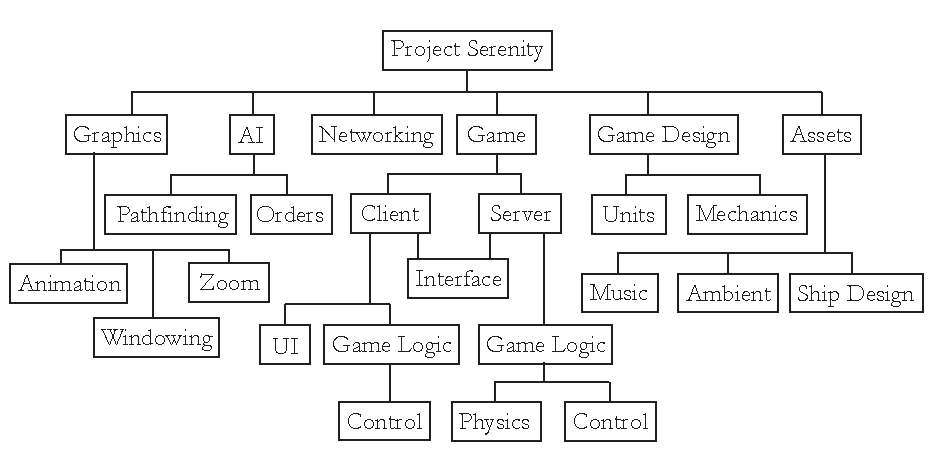
\includegraphics{res/wbs}
	\caption{Work Breakdown Structure of the game components}
\end{figure*}

From the WBS we can further break the project down into components which are suited for weekly development cycles.

Term 2 releases will include a UI, an AI system and further improvements to the components as required. Assets such as music and additional ship designs are non-essential and will likely follow in a later release.

\begin{figure*}
	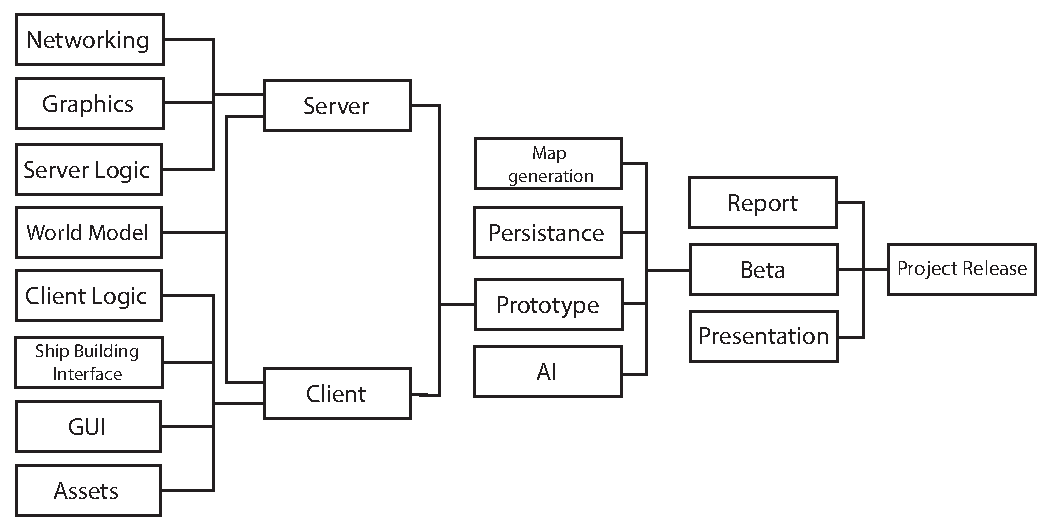
\includegraphics{res/dependency_tree}
	\caption[][-4.3em]{Component Dependency Graph}
\end{figure*}

\begin{figure*}[h!]
	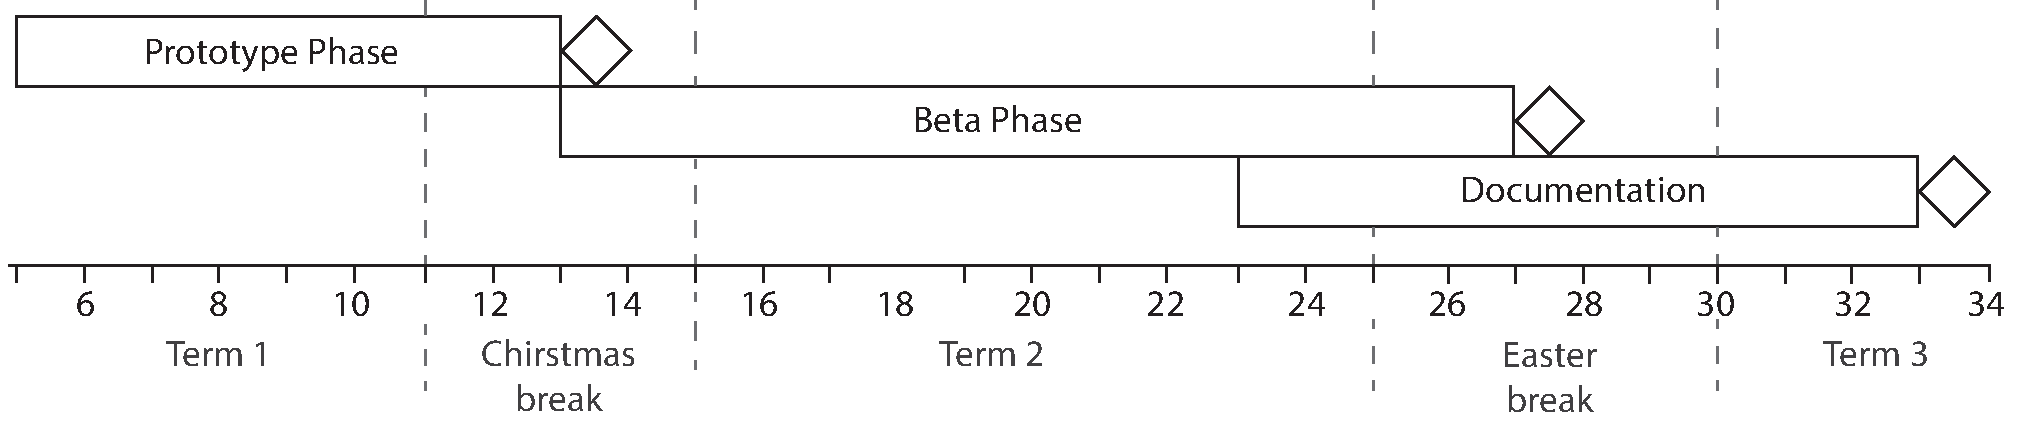
\includegraphics{res/gantt_chart_annotated}
	\caption{Phase level Gantt chart}
\end{figure*}

The dependency tree shows which components are directly dependant on others, and show how delays will propagate through the project. The project dependency diagram shows that potential loss is minimised after a prototype is complete, that is to say there are fewer critical dependancies from the prototype level onwards. This information emphasises the priority of the server and client components should the project schedule require revising at a later stage.





\begin{figure}
	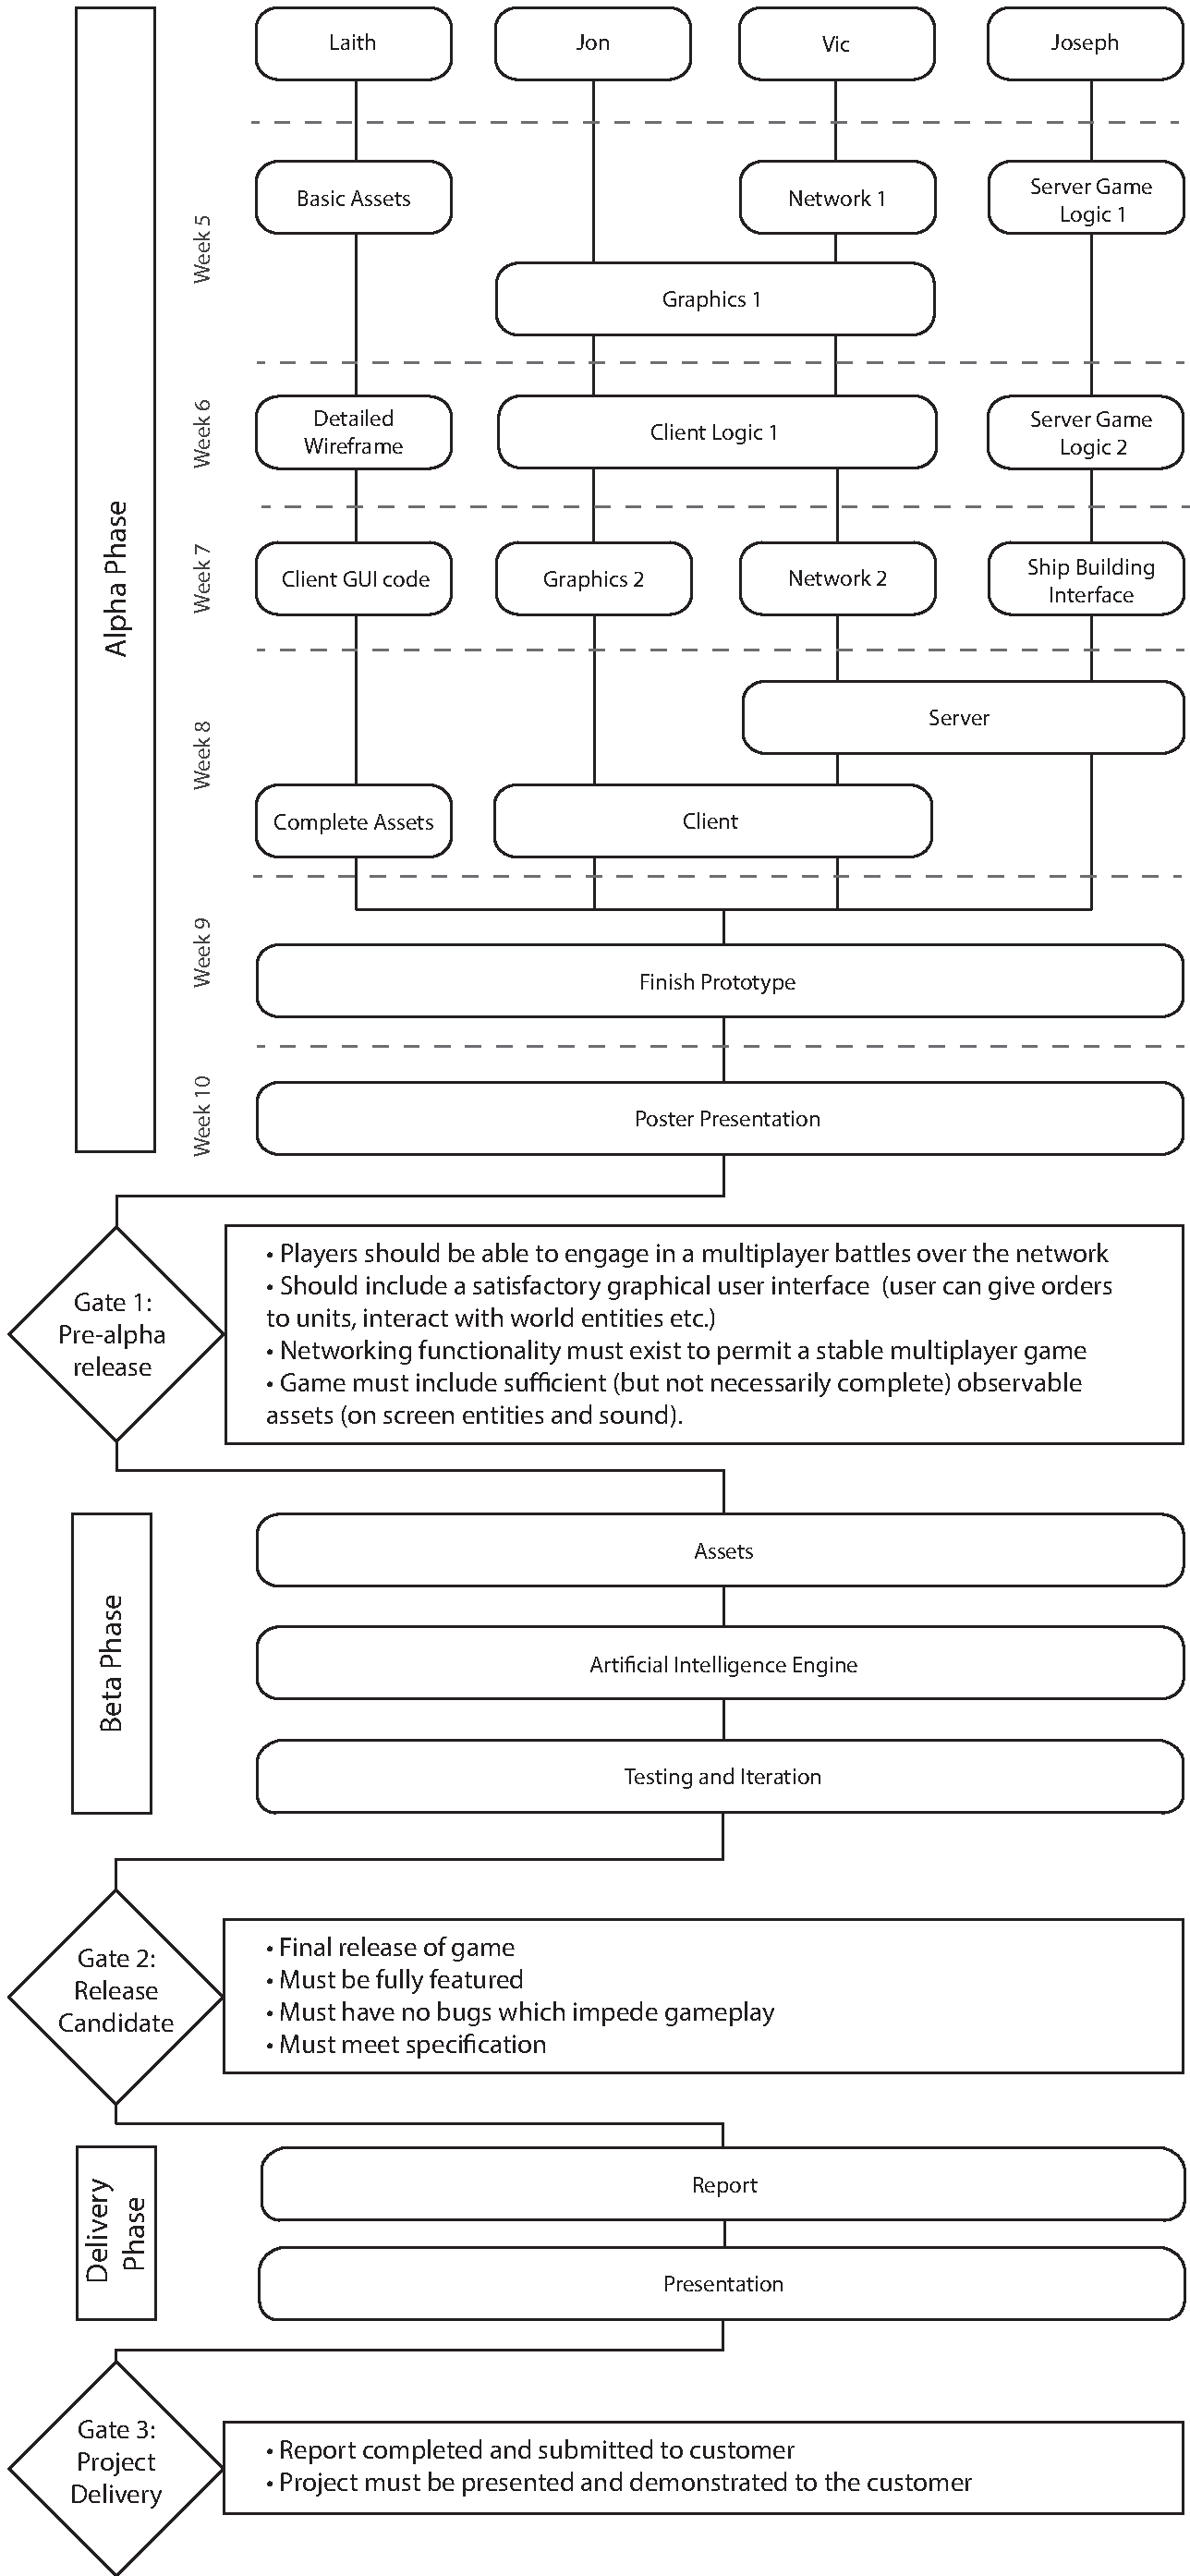
\includegraphics{res/stage_gate_diagram}
	\caption{Stage-gate model of work breakdown structure showing the division of labour across the various project phases. 
	The alpha phase is more thoroughly planned so we are able to see a weekly breakdown of tasks in the near future. The gates are project milestones, each of which details the requirements for proceeding through that gate into the next phase.}
\end{figure}
